\documentclass{beamer}
\usetheme{metropolis}
\usepackage[font=footnotesize, labelfont=footnotesize]{caption}



\title{Introduction}
\subtitle{Wireless Mobile Software Engineering}
\date{21 February 2017}
\author{Steven "Steven"}
\institute{BINUS INTERNATIONAL}


\begin{document}
  \maketitle
  
%  \section {Class organization}
  \begin{frame}{Some basic rules}
  	\begin{itemize}
		\item Phone should be silent at all time
		\item Laptop is fine
		\item Late policy
		\item All slides and handouts are available at github (goo.gl/Lb2VQQ) (Corrections to them are encouraged)
	\end{itemize}
  \end{frame}
  
  \begin{frame}{Who are you?}
	Steven "Steven"
	
		\pause

	Graduated from The University of Edinburgh (2016)
	
	Graduated from Binus International (2012)

		\pause

	Was TA in BI 2010~2012
	
		\pause

	Worked on PT Stampindo Lantjar Jaya
	
	Github profile: https://github.com/SeiryuZ
  \end{frame}
  
  \begin{frame}{My work}
  	Professionally worked on:
	
	\begin{center}
		\begin{figure}
		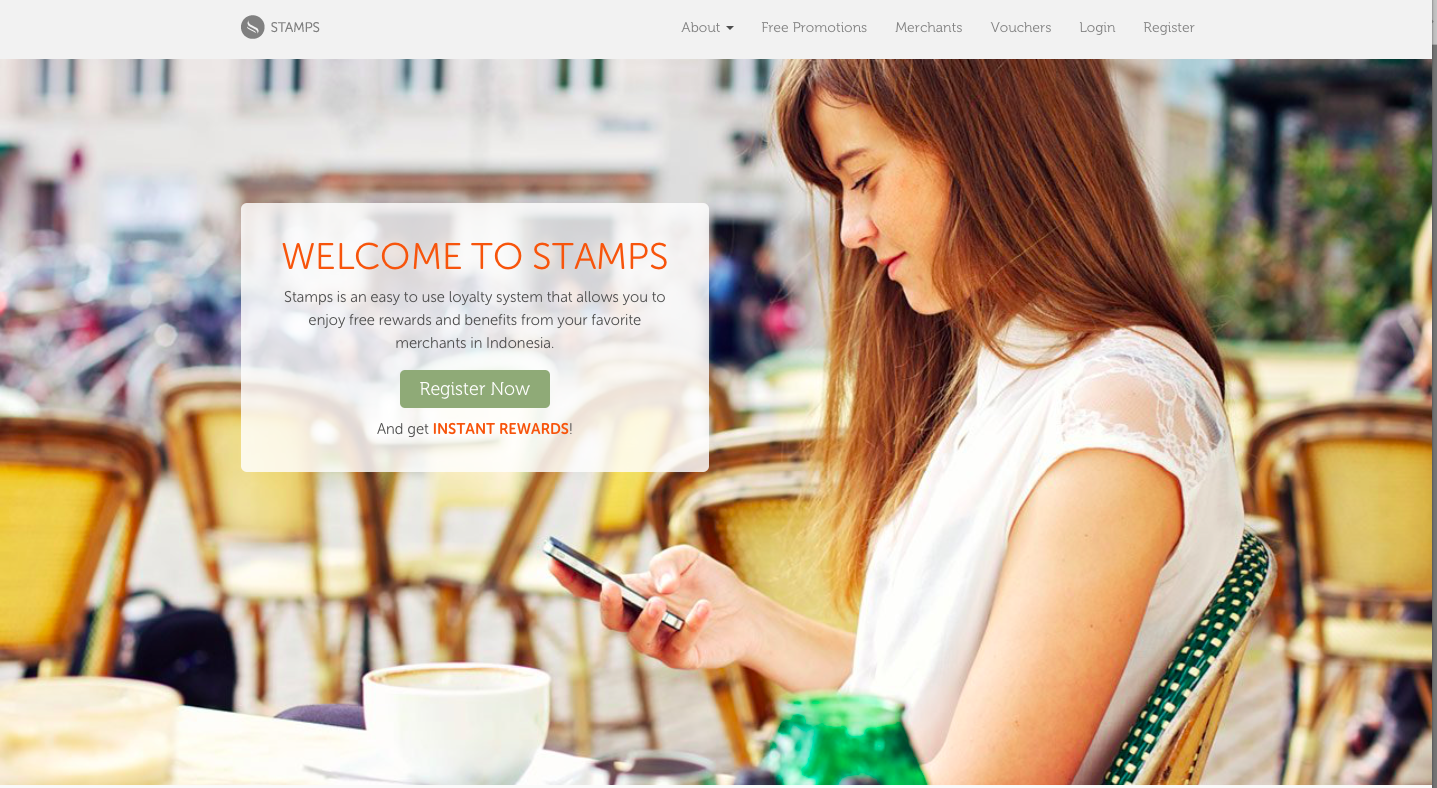
\includegraphics[scale=0.2]{images/stamps.png}
		\caption{stamps.co.id}
		\end{figure}
	\end{center}
  \end{frame}
    \begin{frame}{My work}	
	\begin{center}
		\begin{figure}
		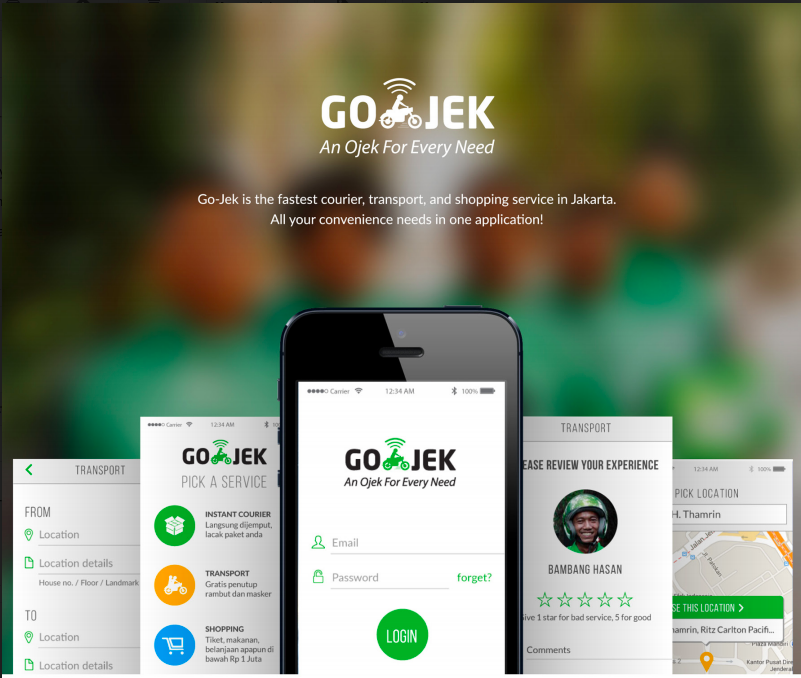
\includegraphics[scale=0.3]{images/gojek.png}
		\caption{GOJEK}
		\end{figure}
	\end{center}
  \end{frame}
    \begin{frame}{My work}
	\begin{center}
		\begin{figure}
		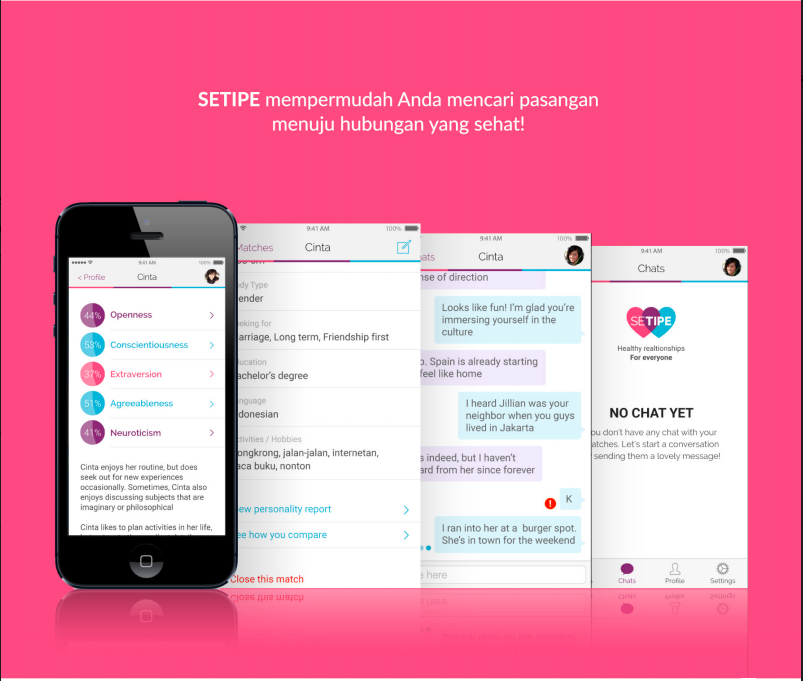
\includegraphics[scale=0.3]{images/setipe.png}
		\caption{setipe.com}
		\end{figure}
	\end{center}
  \end{frame}
    \begin{frame}{My work}
	\begin{center}
		\begin{figure}
		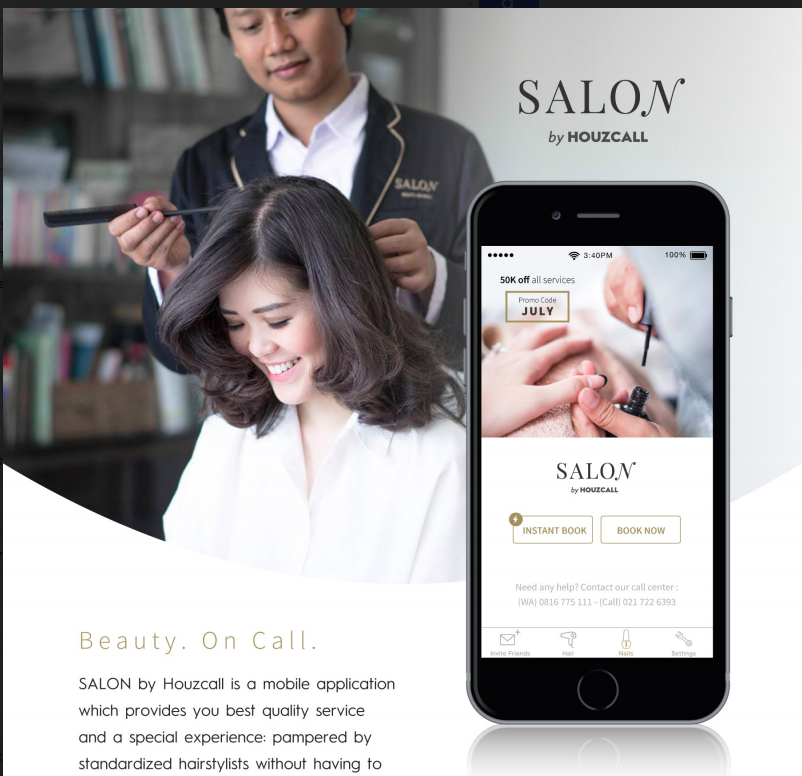
\includegraphics[scale=0.25]{images/salon.png}
		\caption{salon by houzcall}
		\end{figure}
	\end{center}
  \end{frame}
   \begin{frame}{My work}
	\begin{center}
		\begin{figure}
		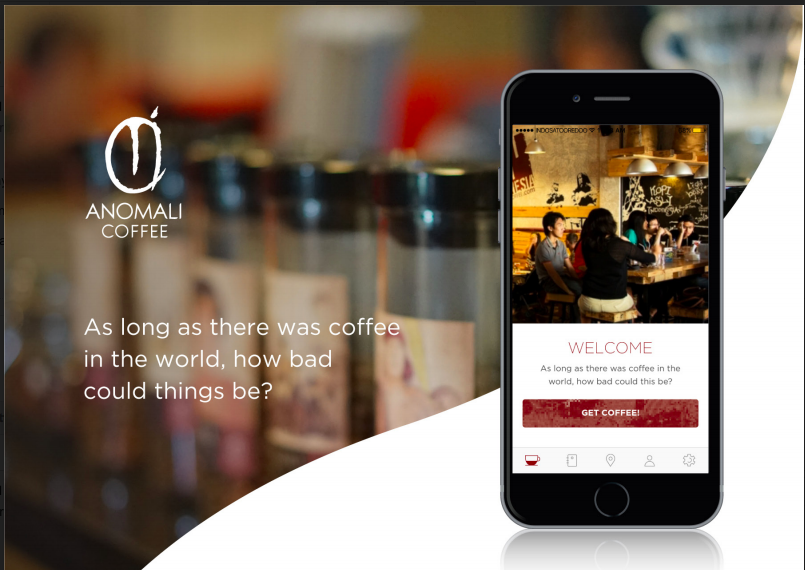
\includegraphics[scale=0.3]{images/anomali.png}
		\caption{Anomali coffee}
		\end{figure}
	\end{center}
  \end{frame}
  
  

  
  
  
    
   \begin{frame}{What are you going to learn in this course}
  	\begin{itemize}
		\item 	Analyze a problem, identify and define the computing requirements appropriate to its solution.
		\item Design and develop an app for the Android mobile computing platform that addresses a social or educational need or business opportunity.n
		\item Apply current techniques, skills, and tools creatively to produce innovative mobile applications.
		\item Demonstrate effective team work to accomplish a common goal.
	\end{itemize}
  \end{frame}
  
  
   \begin{frame}{Class Components}
	\begin{center}
		\begin{figure}
		  % This will be mostly done on github
		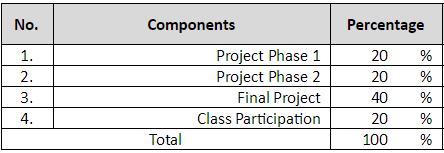
\includegraphics[scale=0.6]{images/class-components.png}
		\caption{Mark breakdown}
		\end{figure}
	\end{center}
  \end{frame}
  
   \begin{frame}{Github-based course}
     \begin{itemize}
     	\item All project will be developed on Github
     	\item Each phase will be its own pull request
     	\item Push your updates early to get comments
     	\item Peer review will be used as class participation mark
     \end{itemize}
     	\begin{center}
		\begin{figure}
		
\includegraphics[scale=0.2]{images/GitHub_Logo.png}
		\end{figure}
	\end{center}
  \end{frame}
    
   \begin{frame}{Some project Ideas}
     \begin{itemize}
     	\item Trojan security app
     	\item Secure Messaging app
     	\item Beautiful Indonesia Wiki
     	\item Home automation mobile app
     \end{itemize}
  \end{frame}
  
    \begin{frame}{Lab today}
     \begin{itemize}

    	\item Configure Android studio to work with your PC / laptop

		\item Make a team of 2 person for your final project
		
		\item Decide on your final project topic
		
		\item \textbf{Due week 2} Draft your project's README.md
		
		Describe what problems you are trying to solve, and  why mobile app is effective? List your development plan (Which feature are you going to finish by phase 1 / 2 / Final presentation)
	\end{itemize}
  \end{frame}
  
  
\end{document}